\documentclass[12pt]{article}
\usepackage{graphicx}
\pagestyle{empty}

\oddsidemargin  -0.5 cm
\evensidemargin 0.0 cm
\textwidth      6.5in
\headheight     0.0in
\topmargin      -1 cm
\textheight=9.0in

\begin{document}

\setlength{\parindent}{0 cm}

\begin{center}
  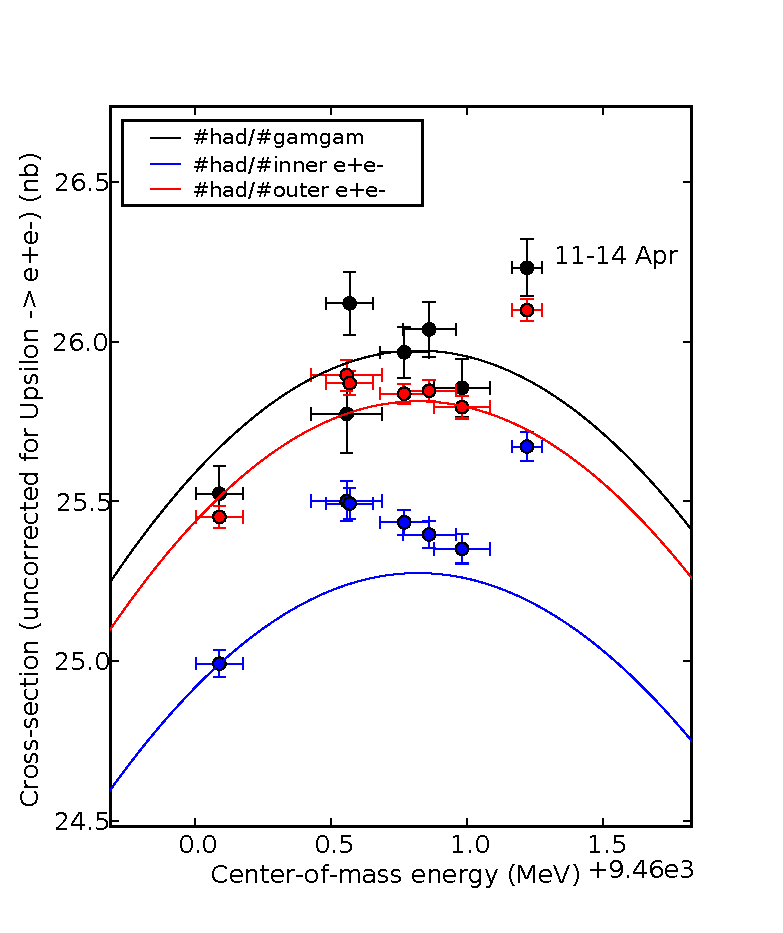
\includegraphics[width=0.9\linewidth]{stability2_thecorrections.eps}
\end{center}

\begin{itemize}

\item These are only peak data, including data past the 48-hour limit,
combined by week (not all $\Upsilon(1S)$ ``weeks'' had peak data).

\item Data $y$-values are ``raw'' cross-section:
\#hadrons/\#$\gamma\gamma$ or $e^+e^-$ without correcting for
$\Upsilon \to e^+e^-$ or beam energy.  Error bars are purely
statistical.

\item Data $x$-values are average beam-energy, corrected for weekly
shifts.  Weekly shifts are determined from $\gamma\gamma$ scan fits,
largely independent of the data plotted here.  Error bars represent
uncertainty from those fits.

\item Black data are \#hadrons/\#$\gamma\gamma$, blue are
\#hadrons/\#inner $e^+e^-$ (0 $<$ $\cos\theta_+$ $<$ 0.6), and red are
\#hadrons/\#outer $e^+e^-$ (0.6 $<$ $\cos\theta_+$ $<$ 0.8).

\item Uppermost curve (black) is the $\gamma\gamma$ fit, only partially
independent of the corresponding (black) data points.

\item Blue and red curves are where we should expect the inner and
outer $e^+e^-$ data to lie (respectively), given the $\Upsilon \to
e^+e^-$ background (with no interference).  The correction has been
put in the curves, rather than the data (where it ultimately belongs).

\item I claim that we observe the $\Upsilon \to e^+e^-$ effect in both
inner and outer $e^+e^-$, including the approximate size of the effect
in the two cases (10--20\% approximate).  (I did this calculation
blind--- it was quite a relief!)  The inner (blue) $e^+e^-$ {\it
should} see a larger contamination from $\Upsilon \to e^+e^-$, and
should have a larger interference term as well.  Perhaps the larger
discrepancy is an interference effect.

\item Data from 14--16 April 2002 are 0.4 nb/26 nb = 1.5\% higher than
the curve.  This agrees with March/April counts from the ntuples
(1.53\%).

\item The width of the peak is fixed by scan data and we have one
point far down the left-hand side of the curve.  The April data would
be high for any value of beam energy, even one that puts it on the top
of the peak (this is mostly noticeable in outer $e^+e^-$, where the
effect was discovered).  {\it The discrepancy is not due to a beam
energy shift.}  (I made this plot because I wasn't sure.  The fact that
it all happens on one week, with a particularly high beam-energy, was
suspicious.)

\item Most interestingly, the discrepancy is common to all three
luminosity measures, meaning that it is due to a systematic error in
hadron counting or a second-biggest shower energy cut (both $e^+e^-$
and $\gamma\gamma$ rely on one, but it's really, really loose for
$e^+e^-$ (40\% beam energy)).

\item Bhabhas and hadrons depend on the same trigger lines and
$\gamma\gamma$ depends on a completely different one, so if the
trigger were at fault, little or no effect would be seen in $e^+e^-$
and $\gamma\gamma$ would have the biggest effect.  That's not what we
see, so I rule out the trigger as a candidate.

\item Bhabhas and hadrons have the same closest track to the origin
cut, and $\gamma\gamma$ has no such thing, so I rule that out for the
same reason.

\item Bhabhas and hadrons share a ``Z event vertex'' cut, but this is
sufficiently complicated that an error might arise only in many-track
environments.  I will consider this.

\item Largest track momentum and visible energy are also both
candidates.

\item The level 3 event filter may also be the cause, but I can't
study it without re-pass2ing raw data.  However, the test is simple:
its efficiency after hadronic cuts ought to be about 99.98\%.  If it
is much lower (say, 98.5\%), it is to blame.  This won't take much
data at all.

\end{itemize}

\end{document}
